\chapter{Multiple-Wave Interference and Gratings}\label{ch:b2:gratings}

Tilt a compact disc under a lamp and it throws a rainbow: its spiral
of pits, a micrometre and a half apart, is a grating --- thousands of
tiny reflecting strips, each sending back a copy of the wave, all
interfering. Two waves give the soft $\cos^2$ fringes of the last
chapters; a thousand give fringes a thousand times narrower, sharp
enough to separate two wavelengths that differ by a part in a hundred
thousand. That is the instrument with which the composition of the
Sun and the speed of galaxies were read, and which sits in every
spectrometer. This chapter adds up $N$ waves, derives the \omterm{prop:b2:gratings:equation}{grating
equation}, its dispersion and its resolving power, and meets the other
multiple-wave device, the Fabry--Pérot cavity that will become the
laser's resonator.

\begin{omfigure}
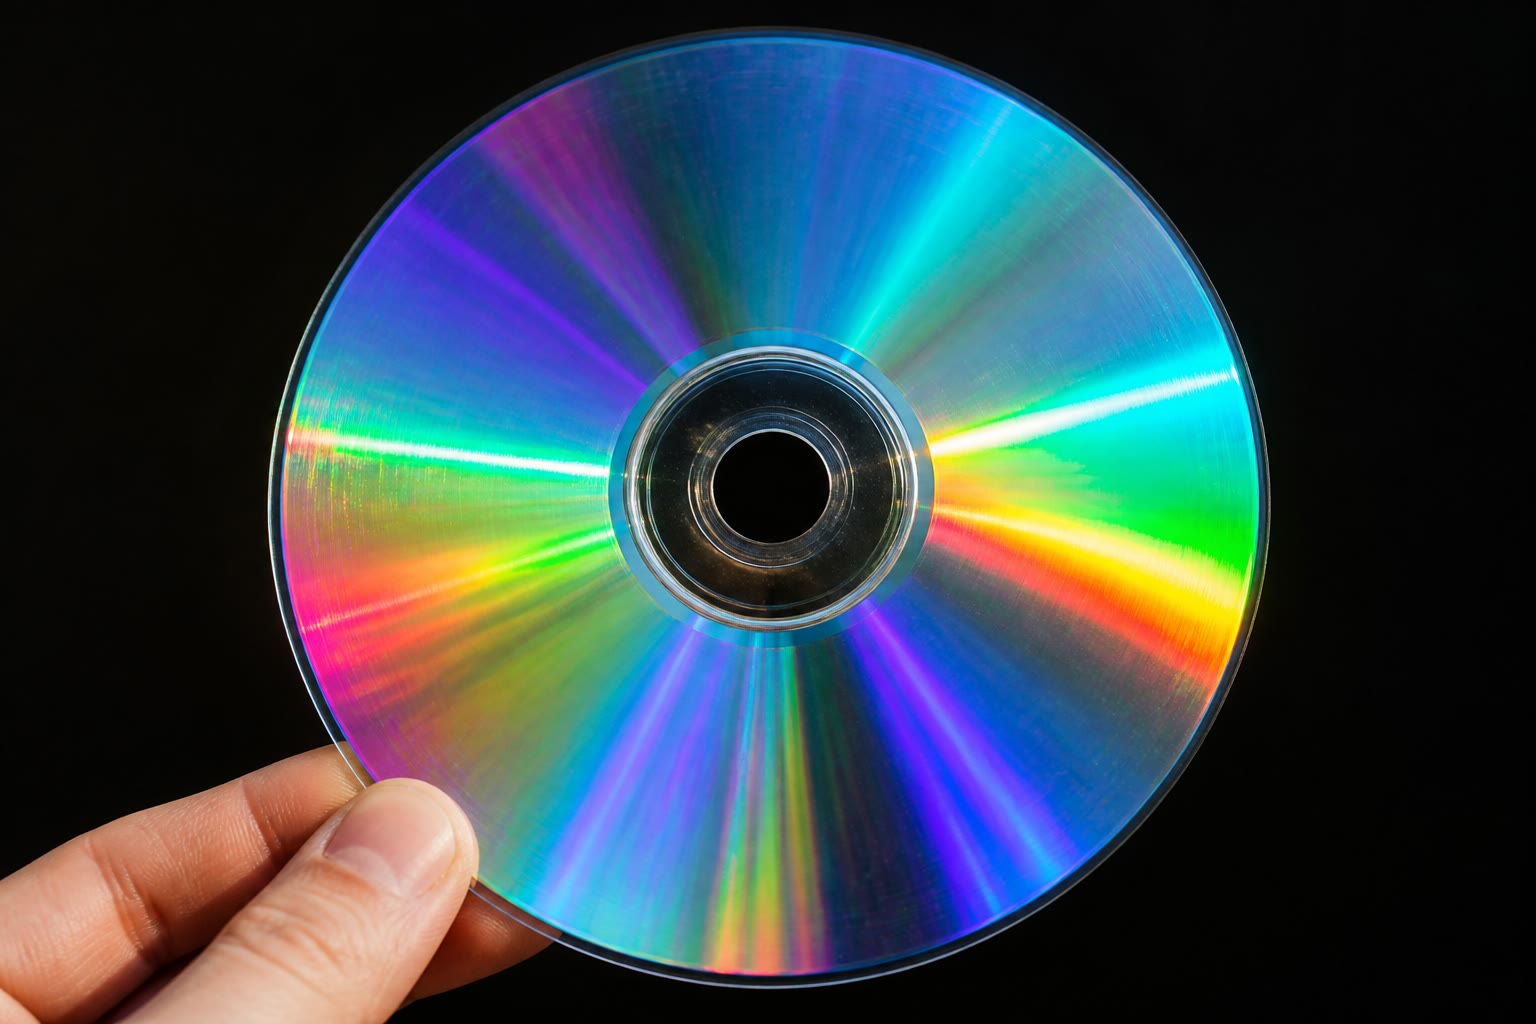
\includegraphics[width=0.54\linewidth]{images/book4/ai/b4-21-cd-diffraction-colours.jpg}

{\small A compact disc in sunlight: its spiral of pits, $\qty{1.6}{\micro m}$ apart, is a reflection grating, and each order spreads the white light into a spectrum.}
\end{omfigure}

\section{Interference of $N$ waves}

\begin{theorem}[$N$ equal waves in arithmetic phase progression]\label{thm:b2:gratings:nwaves}
\index{multiple-wave interference}\index{principal maximum}\index{secondary maximum}\index{phasor}
$N$ coherent waves of equal amplitude $a$, each lagging the previous by
the phase $\varphi$, superpose into a wave of amplitude $A(\varphi)$ and
intensity
\[
A = a\,\frac{\sin(N\varphi/2)}{\sin(\varphi/2)} , \qquad
I(\varphi) = I_0\,\frac{\sin^2(N\varphi/2)}{\sin^2(\varphi/2)} :
\]
\emph{principal maxima} of intensity $N^2I_0$ where $\varphi = 2\pi p$ (all
waves in phase), of angular half-width $2\pi/N$ in $\varphi$ (the first zeros
are at $\varphi = 2\pi p \pm 2\pi/N$), separated by $N - 2$ \emph{secondary
maxima} no higher than about $4.5\%$ of the principal ones for large
$N$. The more waves, the sharper and brighter the peaks: the width
shrinks as $1/N$, the height grows as $N^2$, the energy (their product)
as $N$.
\end{theorem}

\begin{proof}
Complex amplitudes $a\eu^{\iu k\varphi}$, $k = 0, \dots, N - 1$: a geometric
series, $a(1 - \eu^{\iu N\varphi})/(1 - \eu^{\iu\varphi}) = a\eu^{\iu(N - 1)\varphi/2}\sin(N\varphi/2)
/\sin(\varphi/2)$. Zeros where $\sin(N\varphi/2) = 0$ but $\sin(\varphi/2) \ne 0$: $\varphi = 2\pi
m/N$, $m$ not a multiple of $N$. In the phasor picture the $N$ arrows
close into a regular polygon at the zeros and align at the principal
maxima.
\end{proof}

\begin{omfigure}
\begin{tikzpicture}[font=\small, x=1cm, y=1cm, >=Stealth]
  \begin{scope}
    \foreach \k in {0,1,2,3,4} {
      \draw[omDef, thick, ->] ({0.9*sin(\k*36)},{0.9-0.9*cos(\k*36)}) -- ({0.9*sin((\k+1)*36)},{0.9-0.9*cos((\k+1)*36)});
    }
    \draw[omThm, very thick, ->] (0,0) -- ({0.9*sin(180)},{0.9-0.9*cos(180)});
    \node[font=\footnotesize] at (0.3,-0.4) {$N = 5$, $\varphi = 36^\circ$};
    \node[omThm, font=\footnotesize] at (0.45,1.0) {$A$};
  \end{scope}
  \begin{scope}[xshift=3.2cm]
    \foreach \k in {0,1,2,3,4} {
      \draw[omDef, thick, ->] ({0.55*sin(\k*72)},{0.55-0.55*cos(\k*72)}) -- ({0.55*sin((\k+1)*72)},{0.55-0.55*cos((\k+1)*72)});
    }
    \node[font=\footnotesize] at (0.0,-0.4) {$\varphi = 72^\circ$: zero};
  \end{scope}
  \begin{scope}[xshift=9.0cm]
    \begin{axis}[omaxis, axis x line=bottom, axis y line=left, width=7.4cm, height=4.2cm, at={(0,-1.6cm)},
        xlabel={$\varphi/2\pi$}, ylabel={$I/N^2I_0$}, xmin=-0.1, xmax=1.1, ymin=0, ymax=1.08, xtick={0,0.5,1}, ytick={0.5,1}, samples=500,
        xlabel style={at={(axis description cs:0.5,-0.14)}, anchor=north},
        ylabel style={at={(axis description cs:-0.1,0.5)}, rotate=90, anchor=south},
        legend style={font=\scriptsize, at={(0.5,-0.3)}, anchor=north, draw=none, fill=none, legend columns=3}]
      \addplot[omDef, thick, domain=-0.1:1.1] {cos(deg(pi*x))^2};
      \addplot[omThm, thick, domain=-0.1:1.1] {(sin(deg(5*pi*x))/(5*sin(deg(pi*x))+1e-9))^2};
      \addplot[omProp, thick, domain=-0.1:1.1] {(sin(deg(12*pi*x))/(12*sin(deg(pi*x))+1e-9))^2};
      \legend{$N = 2$, $N = 5$, $N = 12$}
    \end{axis}
  \end{scope}
\end{tikzpicture}

{\small Left: the phasor sum of five equal waves --- a regular fan
whose chord is the resultant; it closes into a pentagon, and vanishes,
at $\varphi = 2\pi/5$. Right: the intensity for $2$, $5$ and $12$ waves, normalized
to its peak: the principal maxima sharpen as $1/N$.}
\end{omfigure}

\section{The diffraction grating}

\begin{proposition}[Grating equation]\label{prop:b2:gratings:equation}
\index{diffraction grating}\index{grating equation}\index{order (grating)}\index{angular dispersion}
A \emph{grating} is a set of $N$ identical, equidistant, parallel slits
(or grooves) of period $a$. A plane wave incident at the angle $\theta_0$
from the normal is re-emitted by each slit; in the direction $\theta$ the
waves from neighbouring slits have the \omterm{thm:b2:two-wave-interference:formula}{path difference} $\delta = a(\sin\theta
- \sin\theta_0)$, and they reinforce in the directions
\[
a\,(\sin\theta_p - \sin\theta_0) = p\lambda , \qquad p = 0, \pm1, \pm2, \dots
\]
--- the \emph{orders} of the grating. The zero order is the undeviated
beam for every wavelength; each other order spreads the wavelengths,
with the \emph{\omterm{prop:b2:gratings:equation}{angular dispersion}}
\[
\frac{\dd\theta}{\dd\lambda} = \frac{p}{a\cos\theta} ,
\]
larger for a finer grating and a higher order; the maximum order is
$|p| \le a(1 + |\sin\theta_0|)/\lambda$. A \emph{reflection grating} (grooves ruled
on a mirror) obeys the same equation with the reflected angles.
\end{proposition}

\begin{proof}
The phase between successive slits is $\varphi = 2\pi\delta/\lambda$; the principal
maxima of \cref{thm:b2:gratings:nwaves} are at $\delta = p\lambda$.
Differentiate $a\sin\theta = p\lambda + a\sin\theta_0$ at fixed $p$, $\theta_0$.
\end{proof}

\begin{omfigure}
\begin{tikzpicture}[font=\small, x=1cm, y=1cm, >=Stealth]
  \begin{scope}
    \draw[thick] (0,-1.8) -- (0,-1.3) (0,-1.0) -- (0,-0.5) (0,-0.2) -- (0,0.3) (0,0.6) -- (0,1.1) (0,1.4) -- (0,1.9);
    \foreach \y in {-1.15,-0.35,0.45,1.25} \draw[omDef, thick, ->] (0.1,\y) -- (2.6,{\y+0.9});
    \draw[omDef, thick, ->] (-2.4,0) -- (-0.1,0) node[above, pos=0.4, font=\footnotesize] {$\theta_0 = 0$};
    \draw[dashed] (0.1,-0.35) -- (2.6,-0.35); \draw (1.6,-0.35) arc[start angle=0, end angle=19.8, radius=1.6]; \node[font=\footnotesize] at (1.95,-0.1) {$\theta$};
    \draw[omThm, dashed] (0.1,0.45) -- (0.355,-0.258);
    \draw[omThm, very thick] (0.1,-0.35) -- (0.355,-0.258);
    \node[omThm, font=\footnotesize] at (0.85,-0.6) {$a\sin\theta$};
    \draw[<->] (-0.35,-0.35) -- (-0.35,0.45) node[midway, left, font=\footnotesize] {$a$};
    \node[font=\footnotesize] at (0.8,-2.3) {$a(\sin\theta - \sin\theta_0) = p\lambda$};
  \end{scope}
  \begin{scope}[xshift=8.0cm]
    \draw[thick] (-2.8,0) -- (2.8,0);
    \fill[omExo!70] (-0.2,0.1) rectangle (0.2,0.9); \node[font=\footnotesize] at (0,1.15) {$p = 0$};
    \fill[omDef!70] (0.7,0.1) rectangle (0.95,0.9); \fill[omThm!70] (1.3,0.1) rectangle (1.6,0.9);
    \fill[omDef!70] (-0.95,0.1) rectangle (-0.7,0.9); \fill[omThm!70] (-1.6,0.1) rectangle (-1.3,0.9);
    \node[font=\footnotesize] at (1.15,1.15) {$p = 1$}; \node[font=\footnotesize] at (-1.15,1.15) {$p = -1$};
    \fill[omDef!70] (1.7,0.1) rectangle (2.0,0.9); \fill[omThm!70] (2.5,0.1) rectangle (2.8,0.9); \node[font=\footnotesize] at (2.25,1.15) {$p = 2$};
    \fill[omDef!70] (-2.0,0.1) rectangle (-1.7,0.9); \fill[omThm!70] (-2.8,0.1) rectangle (-2.5,0.9);
    \node[font=\footnotesize, omDef] at (0.8,-0.35) {violet}; \node[font=\footnotesize, omThm] at (1.5,-0.35) {red};
    \node[font=\footnotesize] at (0,-0.9) {spectra of successive orders, spreading with $p$};
  \end{scope}
\end{tikzpicture}

{\small Left: the grating --- neighbouring slits re-emit with the \omterm{thm:b2:two-wave-interference:formula}{path
difference} $a\sin\theta$ at normal incidence. Right: on a screen, the
white zero order and the spectra of the orders $\pm1$, $\pm2$, violet
nearest the centre, wider (and eventually overlapping) as $p$ grows.}
\end{omfigure}

\begin{example}[A classroom grating and a CD]\label{ex:b2:gratings:examples}
A grating of $600$ lines per millimetre ($a = \qty{1.67}{\micro m}$) at normal
incidence sends \qty{500}{nm} light to $\sin\theta = 0.3$, $\theta = \qty{17.5}{\degree}$ in
the first order, $\qty{36.9}{\degree}$ in the second, and has no third order
($3 \times 0.3 > 1$); its first-order spectrum runs from \qty{13.9}{\degree}
(\qty{400}{nm}) to \qty{24.8}{\degree} (\qty{700}{nm}). A compact disc, $a =
\qty{1.6}{\micro m}$, is such a grating in reflection --- hence the rainbow,
and the fact that a DVD ($a = \qty{0.74}{\micro m}$) spreads it wider. The
second-order red (\qty{700}{nm} at $\sin\theta = 0.84$) overlaps the third-order
violet: orders overlap beyond the first, a nuisance cured with filters
or a prism.
\end{example}

\section{Resolving power}

\begin{proposition}[Resolving power of a grating]\label{prop:b2:gratings:resolution}
\index{resolving power (grating)}\index{Rayleigh criterion (spectral)}
Two close wavelengths $\lambda$ and $\lambda + \Delta\lambda$ are just resolved in order $p$
when the \omterm{thm:b2:gratings:nwaves}{principal maximum} of one falls on the first zero of the other
(Rayleigh's criterion), which happens for
\[
\frac\lambda{\Delta\lambda} = pN :
\]
the \emph{resolving power} is the order times the number of lines
lit. It can also be written $W(\sin\theta - \sin\theta_0)/\lambda$ with $W = Na$ the
width of the grating: the largest \omterm{thm:b2:two-wave-interference:formula}{path difference} across the grating,
in wavelengths --- which is why large spectrographs use gratings tens of
centimetres wide and work at grazing angles.
\end{proposition}

\begin{proof}
The maximum of order $p$ for $\lambda + \Delta\lambda$ is at $\varphi = 2\pi p$ for that
wavelength, i.e.\ at $\delta = p(\lambda + \Delta\lambda)$; the first zero of the maximum
for $\lambda$ is at $\delta = p\lambda + \lambda/N$. Equating: $p\Delta\lambda = \lambda/N$. Then $pN =
Na(\sin\theta - \sin\theta_0)/\lambda$.
\end{proof}

\begin{example}[Separating the sodium lines]\label{ex:b2:gratings:sodium}
The doublet, $\Delta\lambda = \qty{0.6}{nm}$ at \qty{589}{nm}, needs $R = 1000$: a
thousand lines in the first order, \qty{2}{mm} of a \qty{600}{lines/mm}
grating. Its own line width, \qty{0.02}{nm}, needs $R = 30\,000$: a \qty{5}{cm}
grating in the first order, or \qty{2.5}{cm} in the second --- and a
\qty{10}{cm} grating of \qty{1200}{lines/mm} in the second order reaches
$240\,000$, resolving \qty{0.0025}{nm}: the width of a line broadened by
the thermal motion of the atoms, and the Doppler shift of a star moving
at \qty{1}{km/s}.
\end{example}

\begin{omfigure}
\begin{tikzpicture}
\begin{axis}[omaxis, axis x line=bottom, axis y line=left, width=8.0cm, height=4.4cm,
    xlabel={$\delta - p\lambda$ (units of $\lambda/N$)}, ylabel={$I$}, xmin=-2.5, xmax=3.5, ymin=0, ymax=1.5, xtick={-2,-1,0,1,2,3}, ytick=\empty, samples=400,
    xlabel style={at={(axis description cs:0.5,-0.14)}, anchor=north},
    ylabel style={at={(axis description cs:-0.06,0.5)}, rotate=90, anchor=south},
    legend style={font=\scriptsize, at={(0.97,0.95)}, anchor=north east, draw=none, fill=none}]
  \addplot[omDef, thick, domain=-2.5:3.5] {(sin(deg(pi*x))/(pi*x+1e-9))^2};
  \addplot[omThm, thick, domain=-2.5:3.5] {(sin(deg(pi*(x-1)))/(pi*(x-1)+1e-9))^2};
  \addplot[black, dashed, domain=-2.5:3.5] {(sin(deg(pi*x))/(pi*x+1e-9))^2+(sin(deg(pi*(x-1)))/(pi*(x-1)+1e-9))^2};
  \legend{$\lambda$, $\lambda + \Delta\lambda$, sum}
\end{axis}
\end{tikzpicture}

{\small Rayleigh's criterion: the peak of one wavelength on the first
zero of the other; the sum (dashed) shows a dip of about $20\%$ between
two resolved lines.}
\end{omfigure}

\section{The Fabry--Pérot cavity}

\begin{proposition}[Multiple-wave interference by division of amplitude]\label{prop:b2:gratings:fabryperot}
\index{Fabry--Pérot interferometer}\index{Airy function}\index{finesse}\index{free spectral range}
Two parallel partially reflecting mirrors (intensity reflectance $R$)
a distance $L$ apart transmit a wave at normal incidence only in so far
as the waves that have bounced $0, 1, 2, \dots$ times between them add
in phase: with $\varphi = 4\pi L/\lambda$ the round-trip phase, the transmitted
intensity is (Airy's function)
\[
\frac{I_t}{I_0} = \frac1{1 + F\sin^2(\varphi/2)} , \qquad F = \frac{4R}{(1 - R)^2} :
\]
sharp peaks of full transmission at $2L = p\lambda$ (the \emph{resonances}
of the cavity, spaced in frequency by the \emph{\omterm{prop:b2:gratings:fabryperot}{free spectral range}}
$c/2L$), of relative width $1/\mathcal F$ with the \emph{finesse} $\mathcal F = \pi
\sqrt R/(1 - R)$ --- $30$ for $R = 0.9$, $300$ for $R = 0.99$. It is the grating's
equal in resolving power ($p\mathcal F$ with $p = 2L/\lambda \sim 10^5$, hence $R \sim
10^7$) and, closed on itself, the resonator of the laser
(\cref{ch:b2:laser}).
\end{proposition}

\begin{proof}
Each round trip multiplies the amplitude by $R\eu^{\iu\varphi}$ (up to a
constant phase); the transmitted amplitude is $t^2a\sum(R\eu^{\iu\varphi})^k =
t^2a/(1 - R\eu^{\iu\varphi})$ with $t^2 = 1 - R$; its squared modulus is $(1 - R)^2/
(1 - 2R\cos\varphi + R^2) = (1 - R)^2/[(1 - R)^2 + 4R\sin^2(\varphi/2)]$. Peaks at
$\varphi = 2\pi p$; half-maximum where $F\sin^2(\varphi/2) = 1$, i.e.\ $\Delta\varphi \approx
4/\sqrt F = 2(1 - R)/\sqrt R$, against the $2\pi$ between peaks.
\end{proof}

\begin{omfigure}
\begin{tikzpicture}
\begin{axis}[omaxis, axis x line=bottom, axis y line=left, width=9.0cm, height=4.4cm,
    xlabel={$\varphi/2\pi$}, ylabel={$I_t/I_0$}, xmin=-0.2, xmax=2.2, ymin=0, ymax=1.1, xtick={0,1,2}, ytick={0.5,1}, samples=800,
    xlabel style={at={(axis description cs:0.5,-0.14)}, anchor=north},
    ylabel style={at={(axis description cs:-0.08,0.5)}, rotate=90, anchor=south},
    legend style={font=\scriptsize, at={(0.5,-0.3)}, anchor=north, draw=none, fill=none, legend columns=3}]
  \addplot[omDef, thick, domain=-0.2:2.2] {1/(1+4*0.3/0.49*sin(deg(pi*x))^2)};
  \addplot[omThm, thick, domain=-0.2:2.2] {1/(1+4*0.8/0.04*sin(deg(pi*x))^2)};
  \addplot[omProp, thick, domain=-0.2:2.2] {1/(1+4*0.95/0.0025*sin(deg(pi*x))^2)};
  \legend{$R = 0.3$, $R = 0.8$, $R = 0.95$}
\end{axis}
\end{tikzpicture}

{\small The Airy transmission of a Fabry--Pérot cavity: full
transmission at the resonances $2L = p\lambda$, peaks narrowing as the
mirrors' reflectance grows.}
\end{omfigure}

\begin{method}[Grating calculations]\label{met:b2:gratings:method}
(1) Period $a = 1/(\text{lines per mm})$; \omterm{prop:b2:gratings:equation}{grating equation} with the
signs of the angles. (2) List the orders that exist ($|\sin\theta| \le 1$)
and check their overlap ($p\lambda_{\max}$ against $(p + 1)\lambda_{\min}$). (3)
Dispersion $p/a\cos\theta$, converted to a position on the detector with
the focal length: $\dd x = f\,\dd\theta$. (4) Resolving power $pN$ with $N$ the
lines actually illuminated; compare $\lambda/R$ with the structure to be
resolved. (5) For real instruments add the entrance slit's width (it
blurs the lines) and the detector's pixels.
\end{method}

\section{Exercises}

\begin{exercise}[$\star$]\label{exo:b2:gratings:1}
A grating of $500$ lines per millimetre at normal incidence, $\lambda =
\qty{550}{nm}$: angles of the orders; highest order; angular width of the
first-order visible spectrum ($400$--\qty{700}{nm}); same grating at
\qty{30}{\degree} incidence: orders on each side.
\end{exercise}

\begin{exercise}[$\star$]\label{exo:b2:gratings:2}
The sodium doublet with a $600$-lines/mm grating and a lens of $f =
\qty{50}{cm}$: angular and linear separation of the two lines on the
detector in the first and second orders; pixel size needed to see
them apart.
\end{exercise}

\begin{exercise}[$\star$]\label{exo:b2:gratings:3}
Resolving power of a \qty{2}{cm} grating of $600$ lines/mm in orders $1$, $2$,
$3$; smallest $\Delta\lambda$ resolved at \qty{550}{nm}; does it separate the sodium
doublet? The hydrogen H$\alpha$ line from its deuterium twin (\qty{0.18}{nm}
apart)?
\end{exercise}

\begin{exercise}[$\star$]\label{exo:b2:gratings:4}
A compact disc ($a = \qty{1.6}{\micro m}$) and a DVD ($a = \qty{0.74}{\micro m}$) lit at
normal incidence: angles of first-order violet and red; which orders
exist for each; why does the CD show two rainbows and the DVD one?
\end{exercise}

\begin{exercise}[$\star\star$]\label{exo:b2:gratings:5}
\emph{The $N$-slit pattern.} (a) Show that between two principal maxima
there are $N - 1$ zeros and $N - 2$ secondary maxima. (b) For large $N$,
intensity of the first \omterm{thm:b2:gratings:nwaves}{secondary maximum} relative to the principal
one (at $N\varphi/2 \approx 3\pi/2$): about $1/22$. (c) Sketch the pattern for
$N = 3$ and $N = 6$ and give the heights of the secondary maxima for
$N = 3$. (d) Fraction of the total energy in the principal maxima for
large $N$ (compare the integrals of the peak, width $\propto 1/N$, height
$\propto N^2$, with the rest).
\end{exercise}

\begin{exercise}[$\star\star$]\label{exo:b2:gratings:6}
\emph{Overlapping orders.} (a) Show that order $p$ of $\lambda_{\max}$ overlaps
order $p + 1$ of $\lambda_{\min}$ when $p\lambda_{\max} > (p + 1)\lambda_{\min}$; for $400$--\qty{700}{nm},
from which order? (b) \omterm{prop:b2:gratings:fabryperot}{Free spectral range} in order $p$: $\Delta\lambda_{\text{FSR}}
= \lambda/p$. (c) A spectrograph works in order $20$ near \qty{500}{nm} (an
echelle grating): \omterm{prop:b2:gratings:fabryperot}{free spectral range}; how is the overlap removed
(cross-disperser)? (d) The Fabry--Pérot's \omterm{prop:b2:gratings:fabryperot}{free spectral range} is $c/2L$:
write it in wavelength and compare with the grating's.
\end{exercise}

\begin{exercise}[$\star\star$]\label{exo:b2:gratings:7}
\emph{Blazed grating.} A reflection grating has its grooves tilted by
the blaze angle $\beta$ so that each facet reflects specularly into the
direction where the order $p$ is wanted. (a) For the Littrow mount
($\theta = \theta_0 = \beta$): show $2a\sin\beta = p\lambda$; blaze angle for first-order
\qty{500}{nm} with $1200$ lines/mm. (b) Why does the blaze send most of the
light into one order (think of the envelope of a single facet's
diffraction, \cref{ch:b2:diffraction})? (c) The same grating is blazed
for \qty{1}{\micro m}: in which order is it efficient at \qty{500}{nm}? (d)
Resolving power of a \qty{10}{cm} grating in Littrow at $\beta = \qty{64}{\degree}$,
$\lambda = \qty{500}{nm}$ (use $R = 2W\sin\beta/\lambda$).
\end{exercise}

\begin{exercise}[$\star\star$]\label{exo:b2:gratings:8}
\emph{The slit.} A spectrometer's entrance slit of width $s$ is imaged
on the detector with magnification $1$; the grating ($600$ lines/mm,
\qty{5}{cm}, order $1$, $f = \qty{50}{cm}$) disperses. (a) Width of a line on
the detector due to the slit alone for $s = \qty{50}{\micro m}$, in nm. (b)
Width due to the grating's resolving power. (c) Which dominates; slit
width at which the two are equal. (d) Why not close the slit further?
\end{exercise}

\begin{exercise}[$\star\star$]\label{exo:b2:gratings:9}
\emph{Fabry--Pérot.} Mirrors $R = 0.95$, $L = \qty{5}{mm}$, $\lambda = \qty{600}{nm}$.
(a) Order $p$, \omterm{prop:b2:gratings:fabryperot}{free spectral range} in frequency and in wavelength. (b)
Finesse; width of a transmission peak in frequency and wavelength. (c)
Resolving power $p\mathcal F$; compare with the \qty{10}{cm} grating. (d) Why
is a Fabry--Pérot always used with a prefilter or a grating?
\end{exercise}

\begin{exercise}[$\star\star\star$]\label{exo:b2:gratings:10}
\emph{The limit of a grating.} (a) Show that $R = pN = W(\sin\theta - \sin\theta_0)
/\lambda \le 2W/\lambda$: the resolving power cannot exceed the width of the
grating in wavelengths, times two. (b) Interpret: the largest \omterm{thm:b2:two-wave-interference:formula}{path
difference} between the extreme rays. (c) A \qty{30}{cm} grating at
\qty{500}{nm}: ultimate $R$; smallest resolvable velocity by Doppler shift
($\Delta\lambda/\lambda = v/c$). (d) Why do astronomers nevertheless reach \qty{1}{m/s}
(think of measuring the position of a line to a fraction of its width,
with many lines)?
\end{exercise}

\begin{exercise}[$\star\star\star$]\label{exo:b2:gratings:11}
\emph{Bragg.} A crystal is a three-dimensional grating: X-rays
reflected by successive atomic planes a distance $d$ apart, at the
glancing angle $\theta$, interfere constructively when $2d\sin\theta = p\lambda$
(Bragg). (a) Derive it from the \omterm{thm:b2:two-wave-interference:formula}{path difference} between two planes.
(b) Copper K$\alpha$ radiation (\qty{0.154}{nm}) on rock salt ($d = \qty{0.282}{nm}$):
the Bragg angles. (c) Why do visible wavelengths give no Bragg
reflection from crystals, and what does the converse (no X-ray
diffraction from glass) tell about glass? (d) Why must $\lambda < 2d$?
\end{exercise}

\begin{exercise}[$\star\star\star$]\label{exo:b2:gratings:12}
\emph{Phased array.} $N$ identical antennas in a line, spaced $a$, fed
with the same amplitude and a phase step $\psi$ between neighbours. (a)
Show that the radiated field in the direction $\theta$ is that of the
$N$-wave sum with $\varphi = 2\pi a\sin\theta/\lambda - \psi$: the main beam points
where $\sin\theta = \lambda\psi/2\pi a$. (b) Half-width of the main beam, $\Delta\theta
\approx \lambda/Na\cos\theta$. (c) Why must $a \le \lambda/2$ to avoid a second main beam
(a grating lobe) when steering? (d) A radar with $64$ elements at
$\lambda/2$, $\lambda = \qty{3}{cm}$: beam width; time to scan $90^\circ$ in steps of one
beam width if the phases switch in \qty{1}{\micro s}.
\end{exercise}

\section{Problem: A spectrograph for a star}

\begin{problem}[{Weekend problem --- designing the spectrograph that
reads a star's light: the grating, the detector, the lines of
hydrogen, and the wobble of a planet}]
\label{pb:b2:gratings:1}

A spectrograph: entrance slit, collimator of focal length $f_1 =
\qty{1.0}{m}$, a reflection grating of $1200$ lines/mm and width $W =
\qty{12}{cm}$, a camera of $f_2 = \qty{1.0}{m}$, a detector with \qty{15}{\micro m}
pixels. It works in the first order, around \qty{550}{nm}, with the
grating at \qty{20}{\degree} incidence.

\medskip
\noindent\textbf{Part I --- The grating.}
\begin{enumerate}
  \item Period of the grating; number of lines lit if the beam covers
        the whole width.
  \item Diffraction angle of \qty{550}{nm} in the first order; of
        \qty{400}{nm} and \qty{700}{nm}; angular width of the visible
        spectrum.
  \item \omterm{prop:b2:gratings:equation}{Angular dispersion} at \qty{550}{nm}; linear dispersion on the
        detector in nm per mm and nm per pixel.
  \item Resolving power; smallest $\Delta\lambda$ resolved at \qty{550}{nm}; in
        pixels.
  \item Does the second-order violet fall onto the first-order
        visible? Which filter removes it?
  \item Length of detector needed for the whole visible spectrum in
        the first order.
  \item The grating is blazed at \qty{17}{\degree}: for which wavelength is
        it most efficient in the first order at this incidence (use
        the Littrow estimate $2a\sin\beta = \lambda$)?
  \item The grating returns $80\%$ of the light at the blaze wavelength
        and the telescope plus optics $40\%$: fraction of the star's
        photons that reach the detector.
\end{enumerate}

\medskip
\noindent\textbf{Part II --- Lines.}
\begin{enumerate}[resume]
  \item The hydrogen Balmer lines of the star: H$\alpha$ \qty{656.3}{nm},
        H$\beta$ \qty{486.1}{nm}, H$\gamma$ \qty{434.0}{nm}: their positions on the
        detector relative to \qty{550}{nm}.
  \item H$\alpha$ from a deuterium atom is \qty{0.18}{nm} shorter: separated?
        By how many pixels?
  \item The sodium doublet in the star's spectrum: separation in
        pixels; and the width of each line if the star's atmosphere
        broadens them to \qty{0.05}{nm}.
  \item The entrance slit is \qty{100}{\micro m} wide, imaged at
        magnification $f_2/f_1$: its width on the detector in pixels and
        in nm; is the spectrograph slit-limited or grating-limited?
  \item The light from the telescope comes as a disc of \qty{1}{''} on
        the sky, which the telescope ($f = \qty{20}{m}$) makes \qty{100}{\micro m}
        wide at the slit: fraction of light lost if the slit is
        narrowed to \qty{50}{\micro m} (take the disc as uniform).
  \item Why does a narrower slit give sharper lines but noisier
        spectra?
\end{enumerate}

\medskip
\noindent\textbf{Part III --- The star moves.}
\begin{enumerate}[resume]
  \item A star recedes at \qty{30}{km/s}: Doppler shift of H$\alpha$ in nm
        and in pixels.
  \item The Earth's orbital motion adds $\pm\qty{30}{km/s}$ over the year:
        why must it be subtracted, and to what precision if one wants
        \qty{100}{m/s}?
  \item A planet makes its star wobble at \qty{10}{m/s}: shift in nm and
        in pixels; is it below the resolution? Explain how measuring
        the centre of a line to a hundredth of its width, over a
        thousand lines, recovers it (statistical gain $\sqrt{N}$).
  \item The temperature of the instrument changes by \qty{1}{K}, and the
        grating (glass, expansion \qty{1e-5}{K^{-1}}) dilates: shift of the
        lines in pixels; what stability is needed for \qty{10}{m/s}?
  \item A calibration lamp (thorium--argon) puts hundreds of known
        lines on the same detector: explain its role.
\end{enumerate}

\medskip
\noindent\textbf{Part IV --- Alternatives.}
\begin{enumerate}[resume]
  \item The same width of grating ruled at $300$ lines/mm and used in
        the fourth order (with a cross-disperser to sort the orders):
        diffraction angle, resolving power, dispersion and \omterm{prop:b2:gratings:fabryperot}{free
        spectral range} at \qty{550}{nm}; what has changed, what has not?
  \item A Fabry--Pérot etalon ($L = \qty{1}{mm}$, $R = 0.9$) placed before
        the slit: \omterm{prop:b2:gratings:fabryperot}{free spectral range} in nm, finesse, peak width; what
        does its comb of transmission peaks look like on the detector,
        and what is it used for?
  \item A prism of \qty{60}{\degree} in glass with $\dd n/\dd\lambda = \qty{-1e-4}{nm^{-1}}$
        has the \omterm{prop:b2:gratings:equation}{angular dispersion} $\dd D/\dd\lambda \approx 2\,\dd n/\dd\lambda$ near
        minimum deviation: compare with the grating's; why did gratings
        replace prisms?
  \item Why are the largest astronomical spectrographs built with
        gratings a metre wide and used at large angles (the limit
        $2W/\lambda$)?
  \item A magnitude-8 star delivers \qty{1e4}{} photons per second and
        per nanometre at the telescope: photons per pixel per second
        on the detector, and the signal-to-noise ratio of a \qty{100}{s}
        exposure (photon noise only).
  \item Summarize: the three numbers that describe a spectrograph
        (dispersion, resolving power, \omterm{prop:b2:gratings:fabryperot}{free spectral range}) and what
        sets each.
\end{enumerate}
\end{problem}
